\documentclass{scrartcl}

\usepackage{riley}
\usepackage{riley-libertine}
\usepackage{riley-euler}


\let\oldepsilon\epsilon
\def\epsilon{\varepsilon}

\usepackage[normalem]{ulem}
\usepackage{tikz}
\newcommand{\dist}{d}
\newcommand{\length}{\mathrm{length}}

\definecolor{graphblue}{rgb}{.4,.4,1}

\begin{document}

\title{Constructing \(\R\) via Cauchy completion}
\author{Riley Levy}
\maketitle{}
This document details how to define the set of real numbers via rational approximations.
\section{Notation}
\begin{itemize}
  \item \(\define\) means defined to be.
  \item \(\N\) is the set of natural numbers \(\{0,1,2,\dots\}\).
  \item \(\Q\) is the rational numbers (quotient).
  \item \(\R\) is the real numbers.
  \item \(\dist(x,y)=\abs{x-y}\) is the distance between the points \(x\) and \(y\).
  \item \(\Q^{\N}\) is the set of sequences of rational numbers
  \item \(\Q^{\N}_{C}\) is the set of rational sequences satisfying \nameref{Cauchy's criterion}
  \item \(\R^{\N}\) is the set of sequences of real numbers
  \item \(\R^{\N}_{C}\) is the set of real sequences satisfying \nameref{Cauchy's criterion}
\end{itemize}
\section{Insufficiency of the rationals}
The discovery of irrational numbers radically changed our concept of a number. It is an ancient discovery, credited to Pythagoras, but it is likely this was discovered independently elsewhere in the world because there are surviving documents with approximations to irrational numbers.

Even in pragmatic mathematics, we're forced to accept irrational numbers as soon as we want to calculate the diagonal of a square:

\[
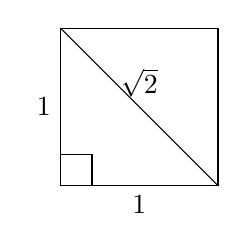
\begin{tikzpicture}[scale=2]
  \draw (0,0) -- node[below]{\(1\)} ++ (1,0);
  \draw (0,0) -- node[left]{\(1\)} ++ (0,1);
  \draw (1,0) -- node[above]{\(\sqrt2\)} (0,1);
  \draw (0,.2) -- (.2,.2) -- (.2,0);
  \draw (1,0) -- (1,1);
  \draw (0,1) -- (1,1);
\end{tikzpicture}
\]

The irrationality of \(\sqrt 2\) would have been understood geometrically at the time, but a modern algebraic proof goes like this:
\begin{theorem}\(\sqrt 2\) is irrational
\end{theorem}
\begin{proof}
  Suppose it is rational. Then there is some fraction \(a/b\) in simplest form where \(a,b\) are integers, \(b\neq 0\), and
  \[
    \paren{\frac a b}^{2}=2.
  \]
  Then
  \begin{align*}
    \frac{a^{2}}{b^{2}} &= 2 \\
    a^{2}&= 2 b^{2}.
  \end{align*}
  Therefore, \(a\) is even. Substitute \(a=2k\). Then
  \begin{align}
    (2k)^{2} &=2 b^{2}. \\
                      \shortintertext{But,}
    4k^{2} &= 2b^{2}, \\
    2k^{2} &= b^{2},
  \end{align}
  proving \(b\) is even too. This contradicts the assumption that \(a/b\) was in simplest form.
\end{proof}

\subsection{What do now?}
How can we work with an irrational number? Relating it back to rational numbers is promising. There are multiple ways to do this. In fact, we defined \(\sqrt 2\) by relating it to \(2\) algebraically: \((\sqrt 2)^2 = 2\). But for this article, an algebraic relationship is of limited use. There is an ambiguity: \((\sqrt 2)^{2} = (-\sqrt 2)^{2} = 2\), so which one did we want?

More damning is the existence of \emph{transcendental numbers}, irrational numbers that are not the solution to any algebraic equation we can spelled using rational numbers, the most famous of which are \(\pi\) and \(e\). Instead, consider \emph{rational approximations}.
In particular, we want approximations that can be made \emph{arbitrarily precise}.
\begin{defn}
  If $x_{n}$ is a sequence approximating $x_{*}$, it can be made arbitrarily precise when, for any desired error tolerance $\epsilon > 0$, there is some large enough $N_{\epsilon}$ that once $n> N_{\epsilon}$, the sequence is within the desired tolerance:
  \[
    n>N_{\epsilon}\implies\dist(x_{n},x_{*}) < \epsilon.
  \]
  Write this
  \[
    \lim_{n\to\infty} x_{n} = x_{*}.
  \]
\end{defn}


\begin{example}[Approximating \(\sqrt 2\) via binary search]
  Binary search is probably the simplest algorithm to approximate \(\sqrt 2\) with arbitrary precision. The idea is to repeatedly bisect an interval containing \(\sqrt 2\) in order to refine our estimate for \(\sqrt 2\).

  To begin, pick an interval \(I_{0}\) containing \(\sqrt 2\), so \(I_{0}=(0,2)\). For our initial estimate, \(x_{0}=1\), take the midpoint of \(I_{0}\). This cuts \(I_{0}\) into its left half, \(L_{0}=I_{0}\cap (-\infty,x_{0})\), and the right half \(R_{0}=I_{0}\cap (x_{0},\infty)\). Then
  \[
    \length(L_{0})=\length(R_{0}) = \frac12 \length(I_{0}) = 1.
  \]
  Observing that \(\sqrt 2\) must lie in one of these halves leads to an error bound:
  \[
    E_{0}\define\dist(x_{0},\sqrt 2) \leq 1.
  \]
  \[
    \begin{tikzpicture}[scale=4]
      \draw[color=graphblue] (0,-.1)node[below]{\(0\)} -- (0,0);
      \draw[color=graphblue] (1,-.1)node[below]{\(1\)} -- (1,0);
      \draw[color=graphblue] (2,-.1)node[below]{\(2\)} -- (2,0);
      \draw (0,0) -- (2,0);
      \fill (1,0)  circle(.5pt) node[above]{\(x_{0}\)};
      \fill (1.414,0)  circle(.5pt) node[below]{\(\sqrt2\)};
      \draw (.5,-.12) node[below]{\(L_{0}\)};
      \draw (1.5,-.12) node[below]{\(R_{0}\)};
    \end{tikzpicture}
  \]
  Now check if we under or over--estimated. Because \({x_{0}}^{2}=(1)^{2}=1\) is less than \(2\), we underestimated; therefore, \(\sqrt 2 \in R_{0}\).

  We can refine this estimate by picking \(I_{1}=R_{1}\) and repeating this process. Take \(x_{1}\) to be its midpoint, \(1.5\). Again, call the left half \(L_{1}=I_{1}\cap (-\infty,x_{1})\) and the right half \(R_{1}=I_{1}\cap (x_{1},\infty)\).
  \[
    \begin{tikzpicture}[scale=4]
      \draw[color=graphblue] (0,-.1)node[below]{\(0\)} -- (0,0);
      \draw[color=graphblue] (1,-.1)node[below]{\(1\)} -- (1,0);
      \draw[color=graphblue] (2,-.1)node[below]{\(2\)} -- (2,0);
      \draw (0,0) -- (2,0);
      \fill (1,0)  circle(.5pt) node[above]{\(x_{0}\)};
      \fill (1.5,0)  circle(.5pt) node[above]{\(x_{1}\)};
      \fill (1.414,0)  circle(.5pt) node[below]{\(\sqrt2\)};
    \end{tikzpicture}
  \]
  The same argument will also give new error bounds. Observe
  \[
    \length( L_{1} ) = \length( R_{1} ) = \frac 1 2 \length( I_{1} ) = \frac{1}{2}.
  \]
  Because \(\sqrt 2\) must lie in one of these halves, we get the error bound
  \[
    E_{1} \define \dist(x_{1},\sqrt 2) \leq \frac 1 2.
  \]
  Checking \({x_{1}}^{2}=2.25 > 2\) shows this time we overestimated, so \(\sqrt 2 \in I_{2}\define L_{0}\).

  In general, given \(I_{n}\), pick \(x_{n}\) to be its midpoint. Let \(L_{n}=I_{n} \cap (-\infty, x_{n})\) be the left half and \(R_{n}=I_{n}\cap (x_{n},\infty)\) be the right half. The lengths of these halves gives an error bound:
  \[
    E_{n} \define \dist(x_{n},\sqrt 2) \leq \length(L_{n}) = \length(R_{n}) = \frac12 I_{n}.
  \]
  Induction on $n$ gives
  \begin{equation}
    E_{n} \leq \frac{1}{2^{n}}.\label{eq:binary search error bound}
  \end{equation}
  Setting
  \[
    I_{n+1} =
    \begin{cases}
      L_{n}& \textrm{if } {x_{n}}^{2} > 2 \textrm{ (overestimated)}\\
      R_{n}& \textrm{if } {x_{n}}^{2} < 2 \textrm{ (underestimated) }
    \end{cases}
  \]
  sets us up for the next iteration.

  \Cref{eq:binary search error bound} is particularly interesting because it shows error can be made arbitrarily small:
  \[
    \lim_{n\to\infty} E_{n} \leq \lim_{n\to\infty}\frac{1}{2^{n}} =0.
  \]
\end{example}

Generalizing this kind of argument leads to a formal definition for the set of real numbers. However, we must take care to avoid circular reasoning. So far, we found this approximation by assuming that some number called \(\sqrt 2\) exists, is well-defined, and works the way we would expect a number to. We can probably patch up this specific approximation in an ad-hoc way, using additional facts about \(\sqrt 2\). But this will not generalize.

\section{Avoiding circularity via Cauchy's criterion}
Our goal is to define a real number as something we can approximate using rational numbers. But how can you tell if you are correctly approximating something that hasn't been defined yet?
Without knowing what \(\sqrt 2\) is, how can we make sense of \(\abs[]{x_{n}-\sqrt 2}\)?

We need to know if a sequence of rational numbers looks like an approximation but without needing to know how to take its limit (or even if its limit exists). That is the purpose of the following test:
\begin{defn}[Cauchy's criterion]\label{Cauchy's criterion}
  A sequence \(x_{n}\) satisfies Cauchy's criterion (``is Cauchy'') when its elements eventually become arbitrarily close:
  \[
    \lim_{i,j\to\infty} d(x_{i},x_{j})=\lim_{i,j\to \infty} \abs{x_{i}-x_{j}} =0
  \]
\end{defn}

Certainly, a convergent sequence passes this test:
\begin{theorem}
  Every convergent sequence satisfies \nameref{Cauchy's criterion}.
\end{theorem}
\begin{proof}
  Recall the triangle inequality:
  \begin{alignat*}{3}
    \dist(x,z)&\leq d(x,y)&&+d(y,z),\\
    \abs{x-z}&\leq \abs{x-y}&&+\abs{y-z}.
  \end{alignat*}

  Suppose the sequence \(x_{\blank}\) has limit \(x_{*}\). Then
  \[
    \lim_{i\to\infty} \dist(x_{i},x_*) = \lim_{j\to\infty} \dist(x_{j},x_{*})=0,
  \]
  hence
  \[
    \lim_{i,j\to\infty} \dist(x_{i},x_{*})+\dist(x_{j},x_{*}) = 0,
  \]
  but
  \begin{alignat*}{3}
    \dist(x_{i},x_{j}) &\leq &&\dist(x_{i},x_{*}) + \dist(x_{j},x_{*}) \\
    \lim_{i,j\to \infty} \dist(x_{i},x_{j}) &\leq \lim_{i,j\to \infty} &&\dist(x_{i},x_{*})+\dist(x_{j},x_{*}) = 0
  \end{alignat*}
\end{proof}
The converse is not always true. There are some Cauchy sequences that have no rational limit. The bisection approximation of \(\sqrt 2\) is one such sequence is an example. I would love to tell you it is Cauchy because it converges---to \(\sqrt 2\). But that is circular reasoning. Instead, I will carefully redefine it and prove it is Cauchy.

\begin{defn}[Bisection approximation to \colorbox{darkgray}{\color{white}{\fontspec{lmmonolt10-bold}{(\,REDACTED\,)}}}]

  Let \(I_{0}\define(0,2)\) be the starting interval. Pick \(x_{n}\) to be the midpoint of \(I_{n}\) (in particular, \(x_{0}=1\)). Let \[H_{n}^{-}\define I_{n}\cap (0,x_{n})\] be the left half of \(I_{n}\) and
  \[H_{n}^{+}\define I_{n}\cap (x_{n},2)\] be the right half.
  Define \(I_{{n+1}}\) by \sout{choosing the half containing \(\sqrt 2\)}
  \[
    I_{{n+1}} \define
    \begin{cases}
      H_{n}^{-}& \textrm{if } x_{n}^{2} < 2 \\
      H_{n}^{+}& \textrm{if } x_{n}^{2} > 2
    \end{cases}
  \]
  The sequence \(n \mapsto x_{n}\) this generates is the desired approximation.
\end{defn}
\begin{theorem}
  The sequence \(n\mapsto x_{n}\) defined above satisfies \nameref{Cauchy's criterion}.
\end{theorem}
\begin{proof}
  As \(H_{n}^{-}\) and \(H_{n}^{+}\) are each halves of \(I_{n}\), their lengths are each half the length of \(I_{n}\):
  \[
    \textrm{length}(I_{n+1}) = \frac 1 2 \textrm{length}(I_{n}).
  \]
  By induction, \[
    \textrm{length}(I_{n}) = \frac{2}{2^{n}}.
  \]
  By construction, whenever \(i,j > n\) both \(x_{i}\) and \(x_{j}\) are contained in \(I_{n}\); therefore,
  \[
    \dist(x_{i},x_{j}) \leq \textrm{length}(I_{n}) = \frac{2}{2^{n}}
  \]
  Taking limits gives
  \[
    \lim_{{i,j}\to\infty} \dist(x_{i},x_{j}) \leq \lim \frac{2}{2^{n}} = 0
  \]
  as desired.
\end{proof}

\begin{theorem}
  The sequence \(n\mapsto x_{n}\) has no limit within the set of rational numbers.
\end{theorem}
\begin{proof}
  Observe that the intervals \(I_{\blank}\) are nested:
  \[
    I_{0} \supset I_{1} \supset I_{2} \supset \dots I_{n} \supset I_{n+1} \supset \dots
  \]
  Fix \(N\). For any \(i> N\), \(x_{i}\in I_{i} \subset I_{N}\). Therefore \(x_{*}\in I_{N}\). But \(N\) was arbitrary, so \(x_{*}\) has to be contained in \(I_{n}\) for all \(n\).

  Write \(I_{n} = (a_{n},b_{n})\). Then \(a_{n}< x_{*} < b_{n}\) and
  \[a_{n}^{2} < x_{*}^{2} < b_{n}^{2}.\]
  Because of how each \(I_{n}\) was chosen \sout{to contain \(\sqrt 2\)}, we are guaranteed that \(a_{n}^{2}< 2 < b_{n}^{2}\). Because the length of \(I_{n}\) approaches \(0\), we find that \(a_{n}-b_{n}\to 0\). Therefore \sout{\(x_{*}=\sqrt 2\)} \(\lim_{{n\to\infty}} a_{n}^{2}=\lim_{{n\to\infty}}b_{n}^{2} = 2\), forcing
  \[
    x_{*}^{2} = 2.
  \]
  There is no such rational number.
\end{proof}

\section{Constructing \(\R\) via equivalence classes of Cauchy sequences}
Multiple sequences can approximate the same number. We need a way to check this that avoids circular reasoning, again without direct reference to the sequences' limit.
\begin{defn}[\(\approx\)]\label{cauchy-eq}
  We say \(\paren{n\mapsto x_{n}}\approx\paren{n\mapsto  y_{n}}\) (or briefly \(x_{n}\approx y_{n}\)) whenever
  \[
    \lim_{{n\to\infty}} \dist(x_{n},y_{n}) = 0.
  \]
\end{defn}

The goal is to use \(\approx\) to collect together equivalent approximations into buckets. These buckets will become our construction of the real numbers. But how do we know they will split cleanly? The necessary property is that \(\approx\) be an \emph{equivalence relation}.
\begin{defn}[Equivalence relation]
  An equivalence relation \(\sim\) must satisfy:
  \begin{enumerate}
    \item reflexivity: \(x\sim x\),
    \item symmetry: \(x\sim y\) is equivalent to \(y\sim x\),
    \item transitivity: if \(x\sim y\) and \(y \sim z\) then \(x\sim z\).
  \end{enumerate}
\end{defn}
\begin{theorem}
  \nameref{cauchy-eq} is an equivalence relation.
\end{theorem}
\begin{proof}
  \phantom{M}
  \begin{enumerate}
    \item Reflexivity follows from noting \(\dist(x,x)=0\). Therefore, if \(n \mapsto x_{n}\) is a Cauchy sequence, \(\dist(x_{n},x_{n})=0\).

    \item Symmetry follows from observing \(\dist\) is symmetric: \(\dist(x,y)=\dist(y,x)\).
    \item Transitivity is a consequence of the triangle inequality.
          If \(x_{n}\approx y_{n}\), then \(\dist(x_{n},y_{n})\to 0\). If \(y_{n}\approx z_{n}\), then \(\dist(y_{n},z_{n})\to 0\). Therefore
          \[
          \dist(x_{n},z_{n}) \leq \dist(x_{n},y_{n}) + \dist(y_{n},z_{n}) \to 0.
          \]
  \end{enumerate}
\end{proof}
Now for the buckets:
\begin{defn}[Equivalence class]
  If \(n\mapsto x_{n}\) is a cauchy sequence, define its \emph{equivalence class}
  \[
    \bracket{n\mapsto x_{n}} \define \set[\big]{n\mapsto y_{n}: \paren{n\mapsto x_{n}}\approx \paren{n\mapsto y_{n}}}.
  \]
  The set of all such equivalence classes is written \(\Q^{\N}_{C}/\approx\).
\end{defn}

We can finally construct the reals!
\begin{defn}
  The set of real numbers is the set of equivalence classes of rational cauchy sequences:
  \[\R \define \Q^\N_{C}/\approx.\]
\end{defn}

We would like to think of the real numbers as containing the rational numbers, so we need to find a copy of \(\Q\) in \(\R\).
\begin{defn}
  Let \(i: \Q \to \R\) via \(i(q) = \bracket{\,\_{} \mapsto q}\), the sequence that is constantly \(q\).
\end{defn}

The basic operations \(+,\times,-,\div,\abs{\cdot}\) extend to \(\R\) similarly:
\[
  \bracket{n\mapsto x_{n}} + \bracket{n\mapsto y_{n}} \define \bracket{n\mapsto x_{n}+y_{n}}.
\]
\begin{theorem}
  The function \(i: \Q \mapsto \R\) is an \emph{isometry} (preserves distance).
\end{theorem}
\begin{proof}
  Consider rational numbers \(x\) and \(y\). Then
  \[
    \dist\paren[\Big]{i(x),i(y)} = \abs[\Big]{\bracket{\,\_{}\mapsto x}- \bracket{\,\_{}\mapsto y}} = \bracket[\Big]{\,\_{}\mapsto \abs{x-y}} = i\paren[\Big]{\dist(x,y)}
  \]
\end{proof}

Now we can define \(\sqrt 2\) by the equivalence class \(\bracket{n\mapsto x_{n}}\) of the sequence \(n\mapsto x_{n}\) found by bisection. We would expect in some sense
\[
  \lim_{{n\to\infty}}x_{n} = \sqrt 2.
\]
We can state this more precisely using \(i:\Q\to\R\) as
\[
  \lim_{n\to\infty}i(x_{n}) = \sqrt 2.
\]
We intuitively interpret the construction of \(\R\) as representing a real number \(r\) by the rational approximations \emph{that converge to \(r\)}. However, until now we haven't formally investigated the convergence of these sequences. The following theorem establishes a formalized version of this intuition as fact.
\begin{theorem}
  If \(n\mapsto x_{n} \in \R=\Q^{\N}_{C}\), then
  \[
    \lim_{n\to\infty} i(x_{n}) = \bracket{n\mapsto x_{n}},
  \]
  \ie{} rational Cauchy sequences converge (in \(\R\)) to the real number they represent.
\end{theorem}
\begin{proof}
  Let \(x_{*}=\bracket{n\mapsto x_{n}}\). It suffices to show
  \[
    \lim_{k\to\infty} x_{*}-i(x_{k}) = 0.
  \]
  Note that the \(0\) in the right hand side is the \emph{real number} \(0\), \ie{}
  \(
    \bracket{\,\_{}\mapsto 0}.
  \)
  But
  \[
    x_{*} - i(x_{k}) = \bracket{n \mapsto x_{n}}-\bracket{\,\_{}\mapsto x_{k}} = \bracket{n\mapsto x_{n}-x_{k}};
  \]
  therefore,
  \[
    \lim_{{k\to\infty}} x_{*}-i(x_{k}) = \lim_{k\to\infty} [n\mapsto x_{n}-x_{k}].
  \]
  Now it suffices to show
  \[
    \lim_{k\to\infty}\paren{n\mapsto x_{n} -x_{k}} \approx \_{}\mapsto0,
  \]
  which follows from observing
  \[
    \lim_{n\to\infty}\lim_{k\to\infty} x_{n}-x_{k} =0
  \]
  by hypothesis that \(n\mapsto x_{n}\) is Cauchy.
\end{proof}
\begin{theorem}
  Every Cauchy sequence of real numbers converges to a real number.
\end{theorem}
\begin{proof}
  Suppose there is an \(n\mapsto x^{(n)}\in \R^{\N}_{C}\). Each \(x^{(n)}\in \R\) so it is represented by some rational cauchy sequence
  \[
    x^{(n)} = \bracket{m\mapsto x^{(n)}_{m}}.
  \]
  Suppose there is an \(n\mapsto x^{(n)}\in \R^{\N}_{C}\). Each \(x^{(n)}\in \R\) so it is represented by some rational cauchy sequence
  \[
    x^{(n)} = \bracket{m\mapsto x^{(n)}_{m}}.
  \]
  Consider the diagonal sequence
  \[
    D\define m\mapsto x^{(m)}_{m}.
  \]
  It suffices to show that
  \[
    \lim_{n\to\infty}x^{(n)} - \bracket{D} = 0,
  \]
  or
  \[
    \lim_{m\to\infty}\lim_{n\to\infty} x^{(n)}_{m}-x^{(m)}_{m} = 0.
  \]


  % By hypothesis, \(x^{(n)}\) is Cauchy, so
  % \[
  %   \lim_{i,j\to\infty} x^{(i)}-x^{(j)} = \lim_{i,j\to\infty} \bracket{m\mapsto x^{(i)}_{m}-x^{(j)}_{m}} =0.
  % \]
  % In particular, \(\lim_{{i,j}\to\infty} x_{m}^{(i)}-x_{m}^{(j)}\approx 0\) implies
  % \[
  %   \lim_{m\to\infty} \lim_{{i,j\to\infty}} x_{m}^{(i)}-x_{m}^{(j)} =0
  % \]
  ???

\end{proof}
\end{document}
